\documentclass[a4paper,titlepage]{article}

\makeatletter
\def\input@path{{../../../template/}{./img}}
\makeatother

\usepackage{Comandi}
\usepackage{Riferimenti}
\usepackage{Stile}

\usepackage{eurosym}
\usepackage{comment}
\usepackage{hyperref}

\def\NOME{Manuale Utente}
\def\VERSIONE{1.0.0}
\def\DATA{2016-08-16}
\def\REDATTORE{Viviana Alessio}
\def\VERIFICATORE{Matteo Franco}
\def\RESPONSABILE{Tommaso Panozzo}
\def\USO{Esterno}
\def\DESTINATARI{\COMMITTENTE \\ & \CARDIN \\ & \PROPONENTE}
\def\SOMMARIO{Manuale destinato agli utenti del \gl{progetto} \PROGETTO\  del gruppo \AUTORE.}


\begin{document}


\maketitle

\begin{diario}
	\modifica{Tommaso Panozzo}{\RES}{Approvazione documento}{2016-08-16}{1.0.0}
	\modifica{Matteo Franco}{\VER}{Verifica documento}{2016-08-12}{0.5.0}
	\modifica{Viviana Alessio}{\PRJ}{Stesura Glossario}{2016-08-12}{0.4.0}
	\modifica{Viviana Alessio}{\PRJ}{Stesura sezione Autenticazione, Edifici, Gioco}{2016-08-11}{0.3.0}
	\modifica{Viviana Alessio}{\PRJ}{Stesura Introduzione}{2016-08-11}{0.2.0}
	\modifica{Viviana Alessio}{\PRJ}{Stesura intestazione e indice documento}{2016-08-10}{0.1.0}
\end{diario}

\newpage
\tableofcontents
\newpage
\listoffigures
\newpage

\section{Introduzione}
	\subsection{Scopo del documento} 
	Questo documento ha lo scopo di spiegare dettagliatamente le strategie secondo cui il gruppo \AUTORE{} intende condurre il \gl{progetto} didattico. 
	\subsection{Scopo del \gl{prodotto}}
	\SCOPO
	\subsection{Glossario}
	\GLOSSARIO
	\subsection{Riferimenti}
		\subsubsection{Normativi}
			\begin{itemize}
				\item \textbf{Capitolato d'appalto C2 - CLIPS:} Communication \& Localisation with Indoor Positioning Systems. \\
				\url{http://www.math.unipd.it/~tullio/IS-1/2015/Progetto/C2.pdf}
				\item \textbf{Vincoli e dettagli tecnico-economici} \\
				\url{http://www.math.unipd.it/~tullio/IS-1/2015/Dispense/PD01.pdf}
				\item \textbf{Norme di Progetto} \\ \NPdoc
				\item \textbf{Regolamento di Progetto} \\
				\url{http://www.math.unipd.it/~tullio/IS-1/2015/Progetto/}
				\item \textbf{Regolamento organigramma} \\
				\url{http://www.math.unipd.it/~tullio/IS-1/2015/Progetto/PD01b.html}
			\end{itemize}	
			
		\subsubsection{Informativi}
			\begin{itemize}
				\item \textbf{Software Engineering (10th edition}) \\
				Ian Sommerville \\
				Pearson Education | Addison-Wesley
				\item \textbf{Guide to the Software Engineering Body of Knowledge}
				IEEE Computer Society. Software Engineering Coordinating Committee
				\item \textbf{Slides del \COMMITTENTE} \\ riguardo i  \href{http://www.math.unipd.it/~tullio/IS-1/2015/Dispense/L02.pdf}{processi \gl{software}}, il \href{http://www.math.unipd.it/~tullio/IS-1/2015/Dispense/L03.pdf}{ciclo di vita del \gl{software}} e \href{http://www.math.unipd.it/~tullio/IS-1/2015/Dispense/L04.pdf}{la gestione di \gl{progetto}}	
			\end{itemize}
	\subsection{Modello di ciclo di vita scelto}
	È stato scelto come ciclo di vita il modello \gl{incrementale}. Le motivazioni che ci hanno spinto verso questa direzione sono il modo in cui è strutturato il \gl{progetto} didattico e la quasi totale inesperienza dei componenti del gruppo nello sviluppare progetti \gl{software} di grandi dimensioni. Di seguito una lista di caratteristiche del metodo \gl{incrementale}:
	\begin{itemize}
		\item si può produrre valore ad ogni incremento;
		\item ogni incremento riduce il rischio di fallimento;
		\item prevede rilasci multipli;
		\item i requisiti utente sono classificati e trattati in base alla loro importanza strategica. I requisiti più importanti sono già stabili all'inizio dello sviluppo del \gl{progetto};
		\item l'analisi dei requisiti e la progettazione architetturale non vengono ripetute;
		\item prima si pensa allo sviluppo dei requisiti essenziali, poi a quelli desiderabili;
		\item Sono presenti delle iterazioni del tipo Prototipo $\rightarrow$ Validazione $\rightarrow$ Prototipo $\rightarrow$ Validazione $\rightarrow$ ecc..
	\end{itemize}
	\subsection{Scadenze}
	Il gruppo Beacon Strips ha deciso di rispettare le seguenti scadenze:
	\begin{itemize} 
		\item \textbf{Revisione dei Requisiti}: 2016-04-18
		\item \textbf{Revisione di Progettazione}: 2016-06-17
		\item \textbf{Revisione di Qualifica}: 2016-08-24
		\item \textbf{Revisione di Accettazione}: 2016-09-12
	\end{itemize}
	In base a queste scadenze e a fronte dell'analisi dei rischi verranno decise le fasi in cui suddividere il lavoro di sviluppo del \gl{progetto}.
	\subsubsection{Scelta Revisione di Progettazione}
	Si è deciso di affrontare la RP$_{\mbox{\textit{min}}}$. Il gruppo si impegna quindi per il 2016-06-17 di presentare nel documento ``Specifica Tecnica'' la progettazione ad alto livello del \gl{prodotto}.
	

\section{Requisiti di Sistema} 
L'applicazione da noi realizzata può essere eseguita solamente su dispositivi \gl{mobile} con sistema operativo \gl{Android} di versione uguale o superiore alla 5.0 (Lollipop, \gl{API 21}. \\
Il dispositivo mobile in uso deve inoltre avere attivi i seguenti servizi:
\begin{itemize}
	\item GPS
	\item internet
	\item bluetooth
\end{itemize} 

\subsection{Installazione}

Prima di poter installare l'applicazione è necessario attivare l'opzione "Origini sconosciute" nelle impostazioni.
Per attivare tale opzione è necessario:
\begin{itemize}
	\item andare in Impostazioni
	\item selezionare Sicurezza
	\item attivare "Origini sconosciute"
\end{itemize}


Una volta che ci si è assicurati di avere l'opzione "Origini sconosciute" attiva è necessario visitare il sito \url{http://beaconstrips.tk} e premere sul tasto "Download" che si trova verso il fondo della pagina.


Una volta scaricato il file è necessario premere sulla notifica del completamento del download per far partire il processo di installazione. Infine seguire le istruizioni a schermo per completare il processo.

\subsubsection{Aggiornamento}

Per aggiornare l'applicazione è sufficiente seguire i passi precedentemente descritti. Una volta premuto sulla notifica del completamento del download vi verrà chiesto se volete aggiornare l'applicazione. Premere sì e proseguire con le istruzioni a schermo per completare il processo.

\section{Utilizzo dell'applicazione}
\subsection{Informazioni generali}
Tutte le funzionalità dell'applicazione sono accessibili dal menu laterali apribile tramite uno \gl{swipe} da sinistra verso destra oppure cliccando sul bottone \gl{Hamburger button} presente in alto a sinistra. 

\begin{figure}[!h]
	\centering
	
\includegraphics[scale=0.2]{screenshot/menu_before}
	\caption{Hamburger button}
\end{figure}

\begin{figure}[!h]
	\centering
	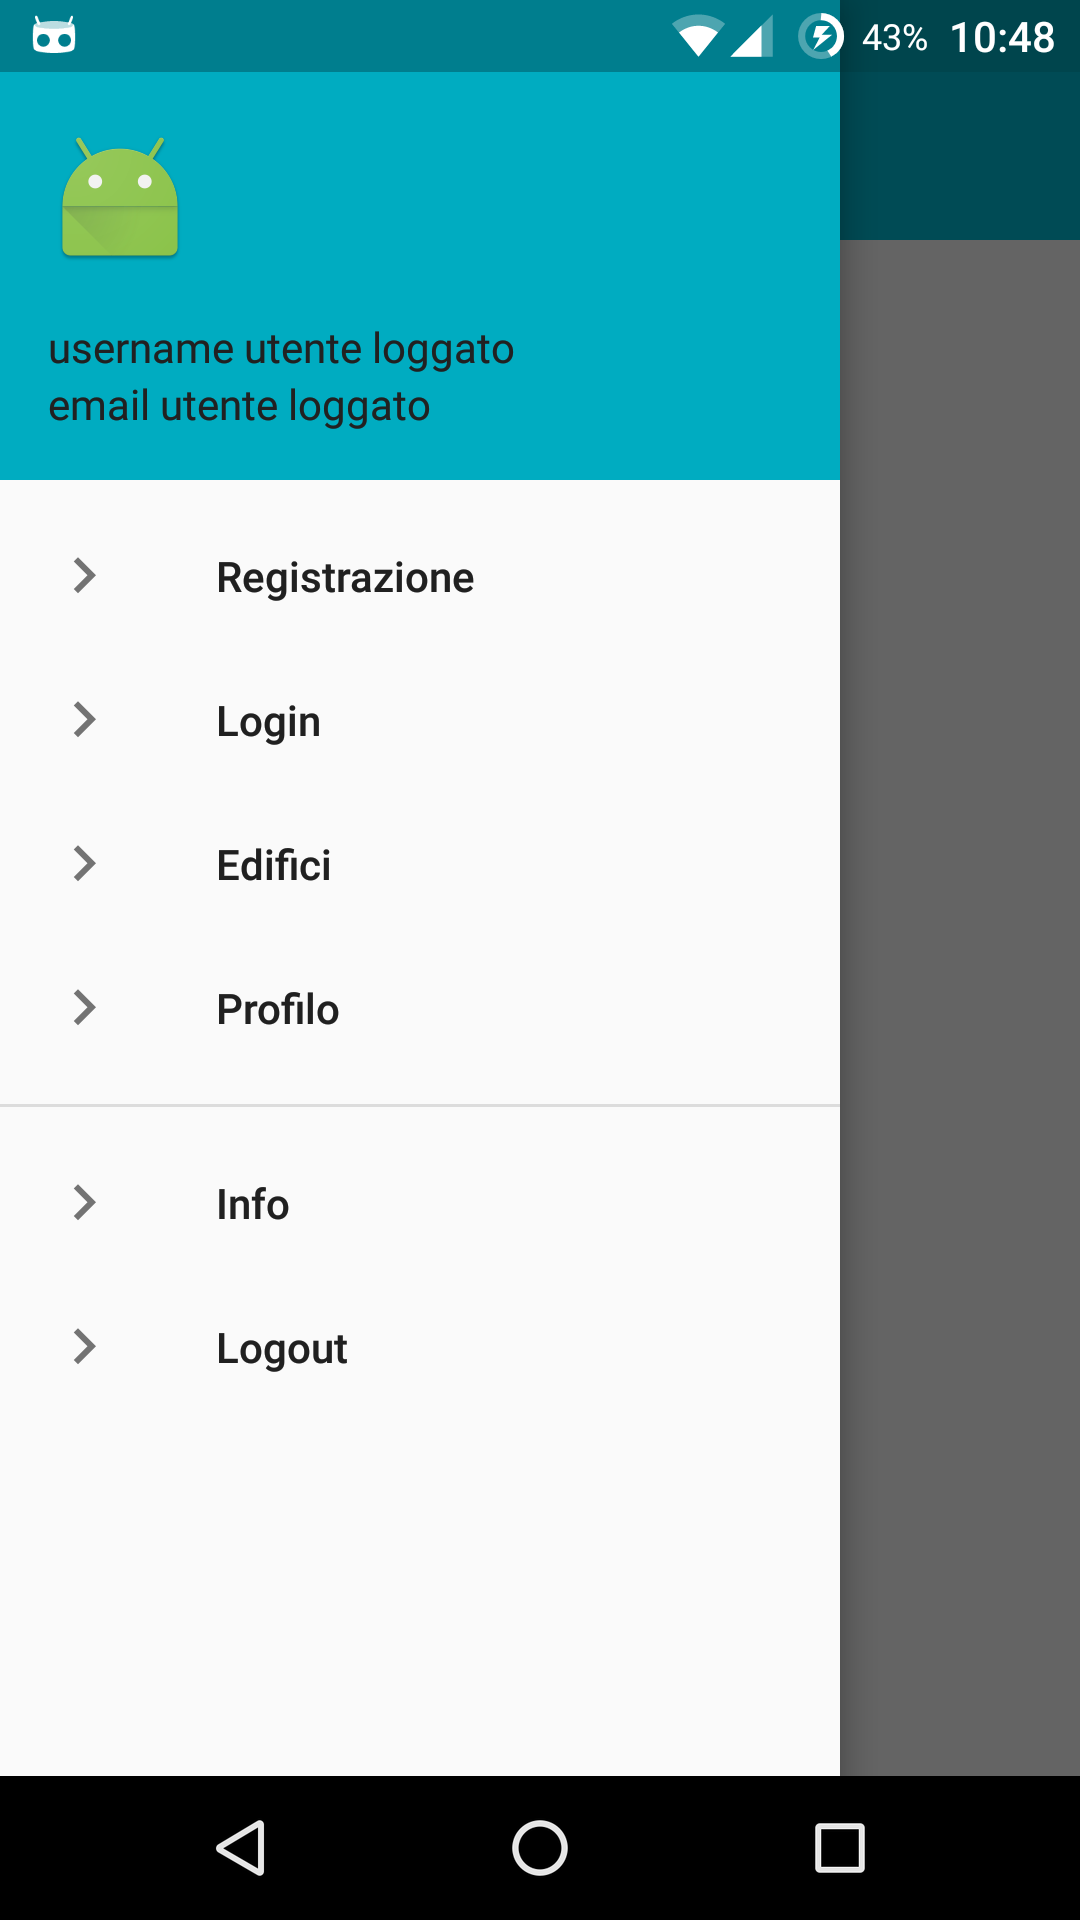
\includegraphics[scale=0.15]{screenshot/menu}
	\caption{Visualizzazione menu aperto}
\end{figure}

\subsection{Autenticazione} 
\subsubsection{Registrazione}

\begin{figure}[!h]
	\centering
	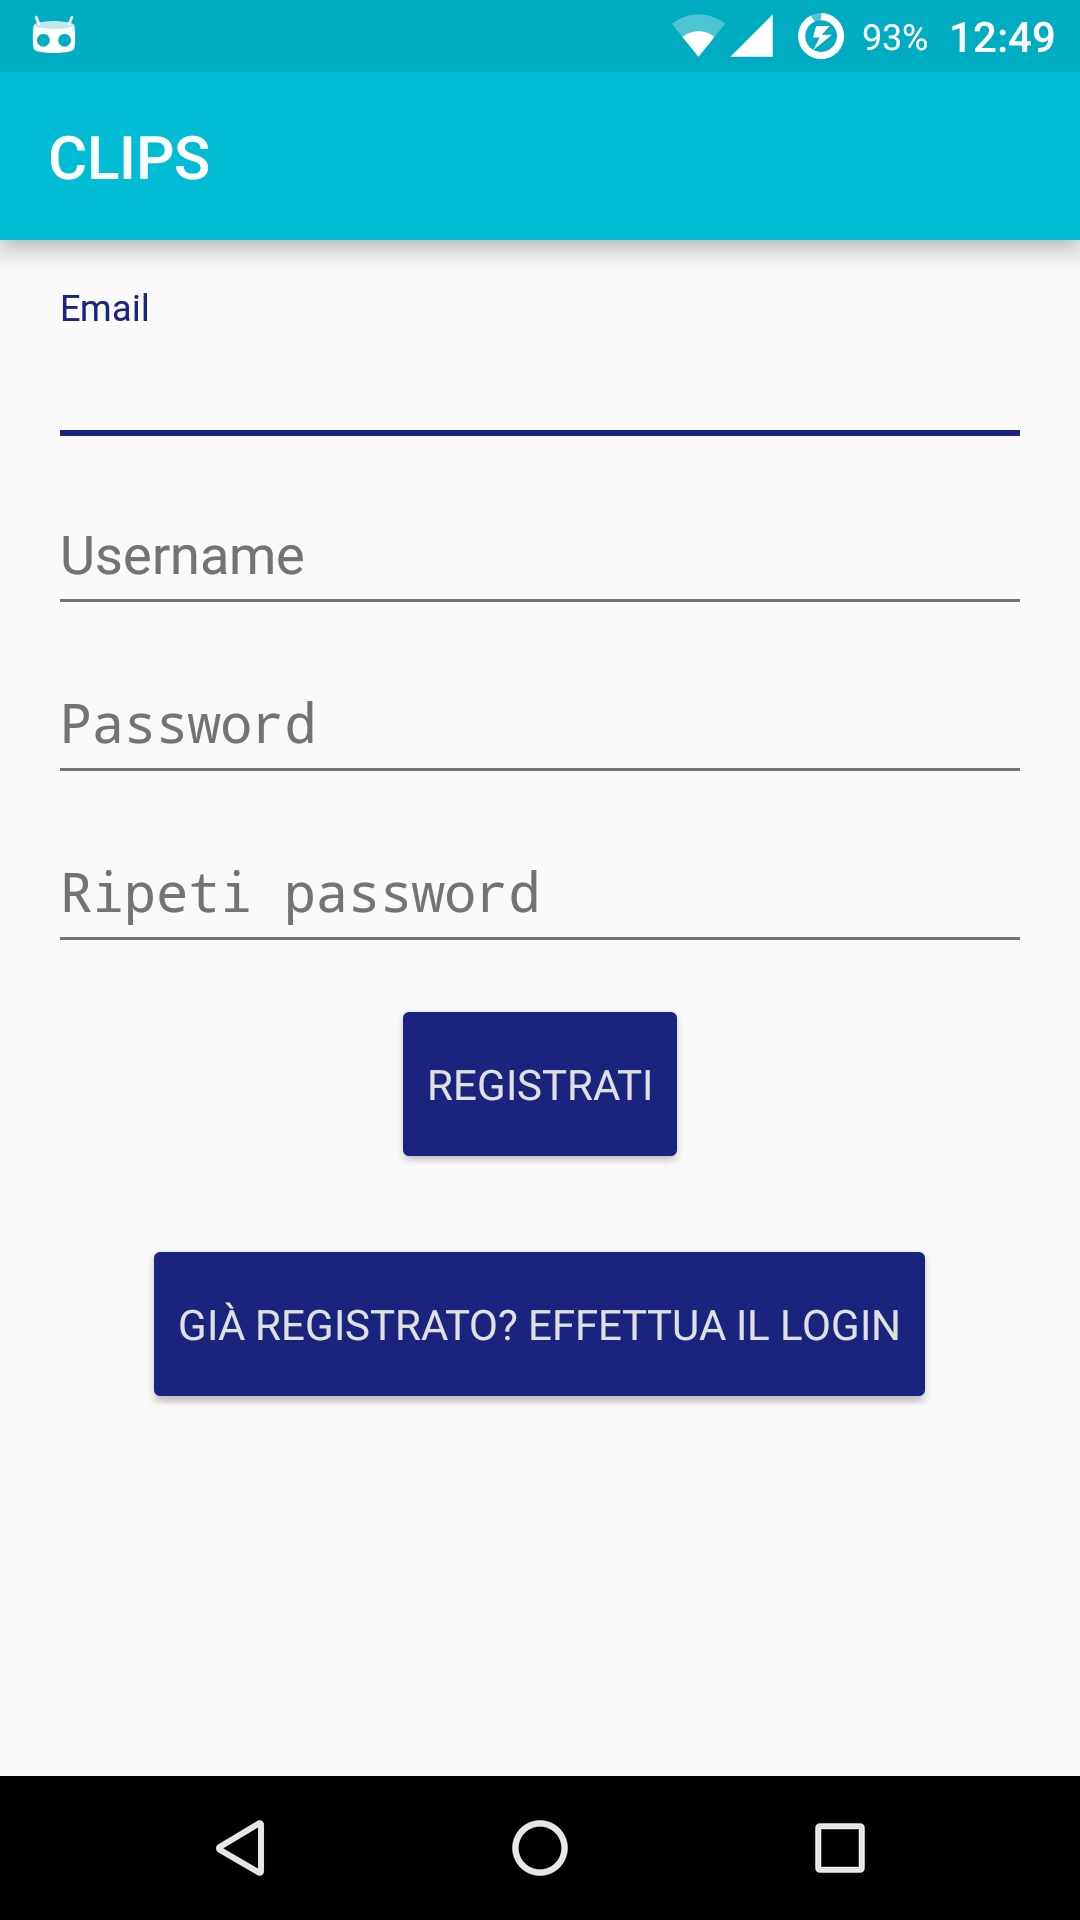
\includegraphics[scale=0.15]{screenshot/Registrazione}
	\caption{Schermata di registrazione}
\end{figure}

Attraverso questa schermata l'utente deve inserire nella form tutti i dati richiesti e successivamente potrà registrarsi cliccando l'apposito bottone ``REGISTRATI''. Successivamente verrà automaticamente autenticato nel sistema.
\subsubsection{Login}
\begin{figure}[!h]
	\centering
	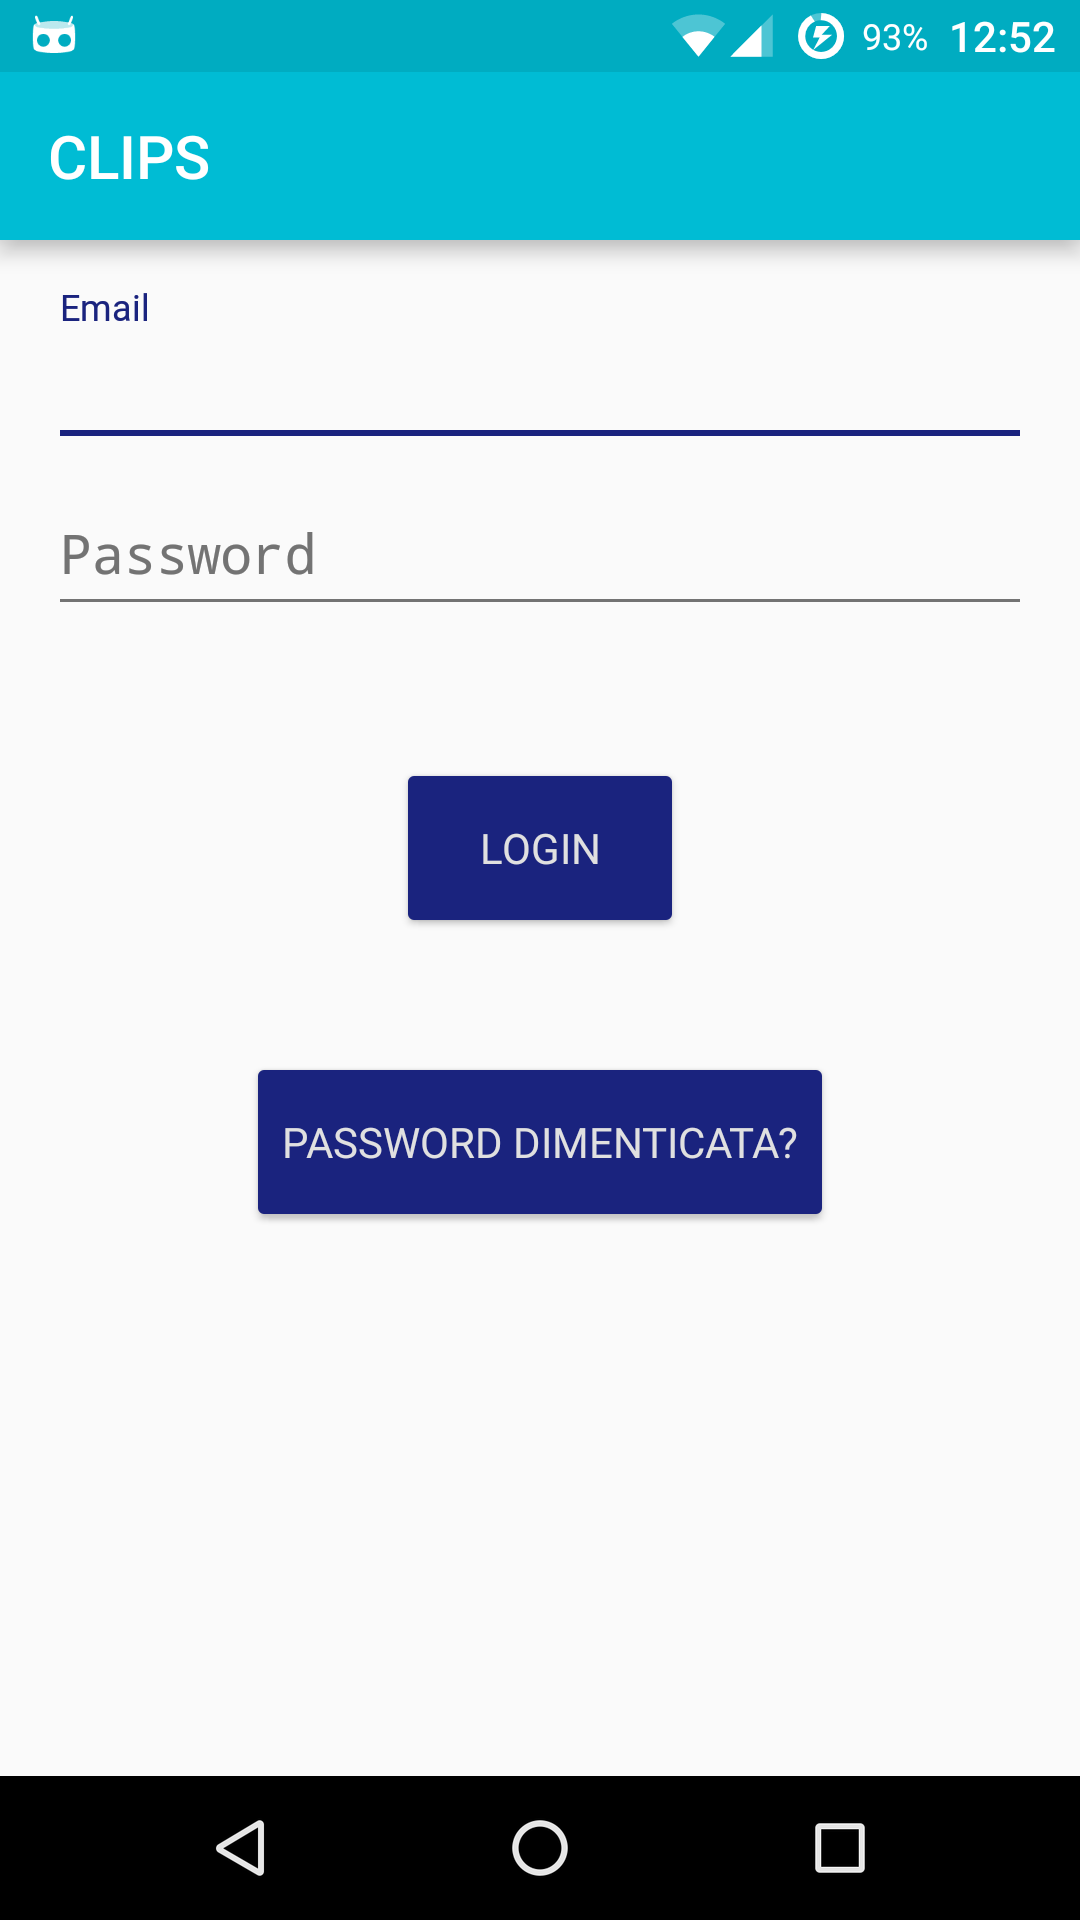
\includegraphics[scale=0.15]{screenshot/login}
	\caption{Schermata di registrazione}
\end{figure}
Qualora un utente si fosse già registrato nel sistema può accedere a questa schermata che gli consentirà, inserendo Email e Password di accedere al sistema.
\newpage


\subsubsection{Account}


\section{Edifici}
\subsection{Ricerca di un edificio}
Da questa schermata l'utente può provare a cercare edifici intorno a sè. \\ Cliccando il \gl{checkbox} ``Ricerca per raggio'' e poi muovendo lo \gl{slider} sottostante può decidere in che raggio di distanza cercare edifici. Una volta cliccato il pulsante ``CERCA EDIFICI NEL RAGGIO SELEZIONATO'' compariranno al di sotto dello stesso bottone la lista degli edifici presenti nel raggio selezionato. \\ 
Successivamemte basterà cliccare sull'edificio desiderato per accedere alla schermata in cui vengono visualizzate informazioni riguardo l'edificio e i percorsi disponibili nell'edificio stesso.
\begin{figure}[!h]
	\centering
	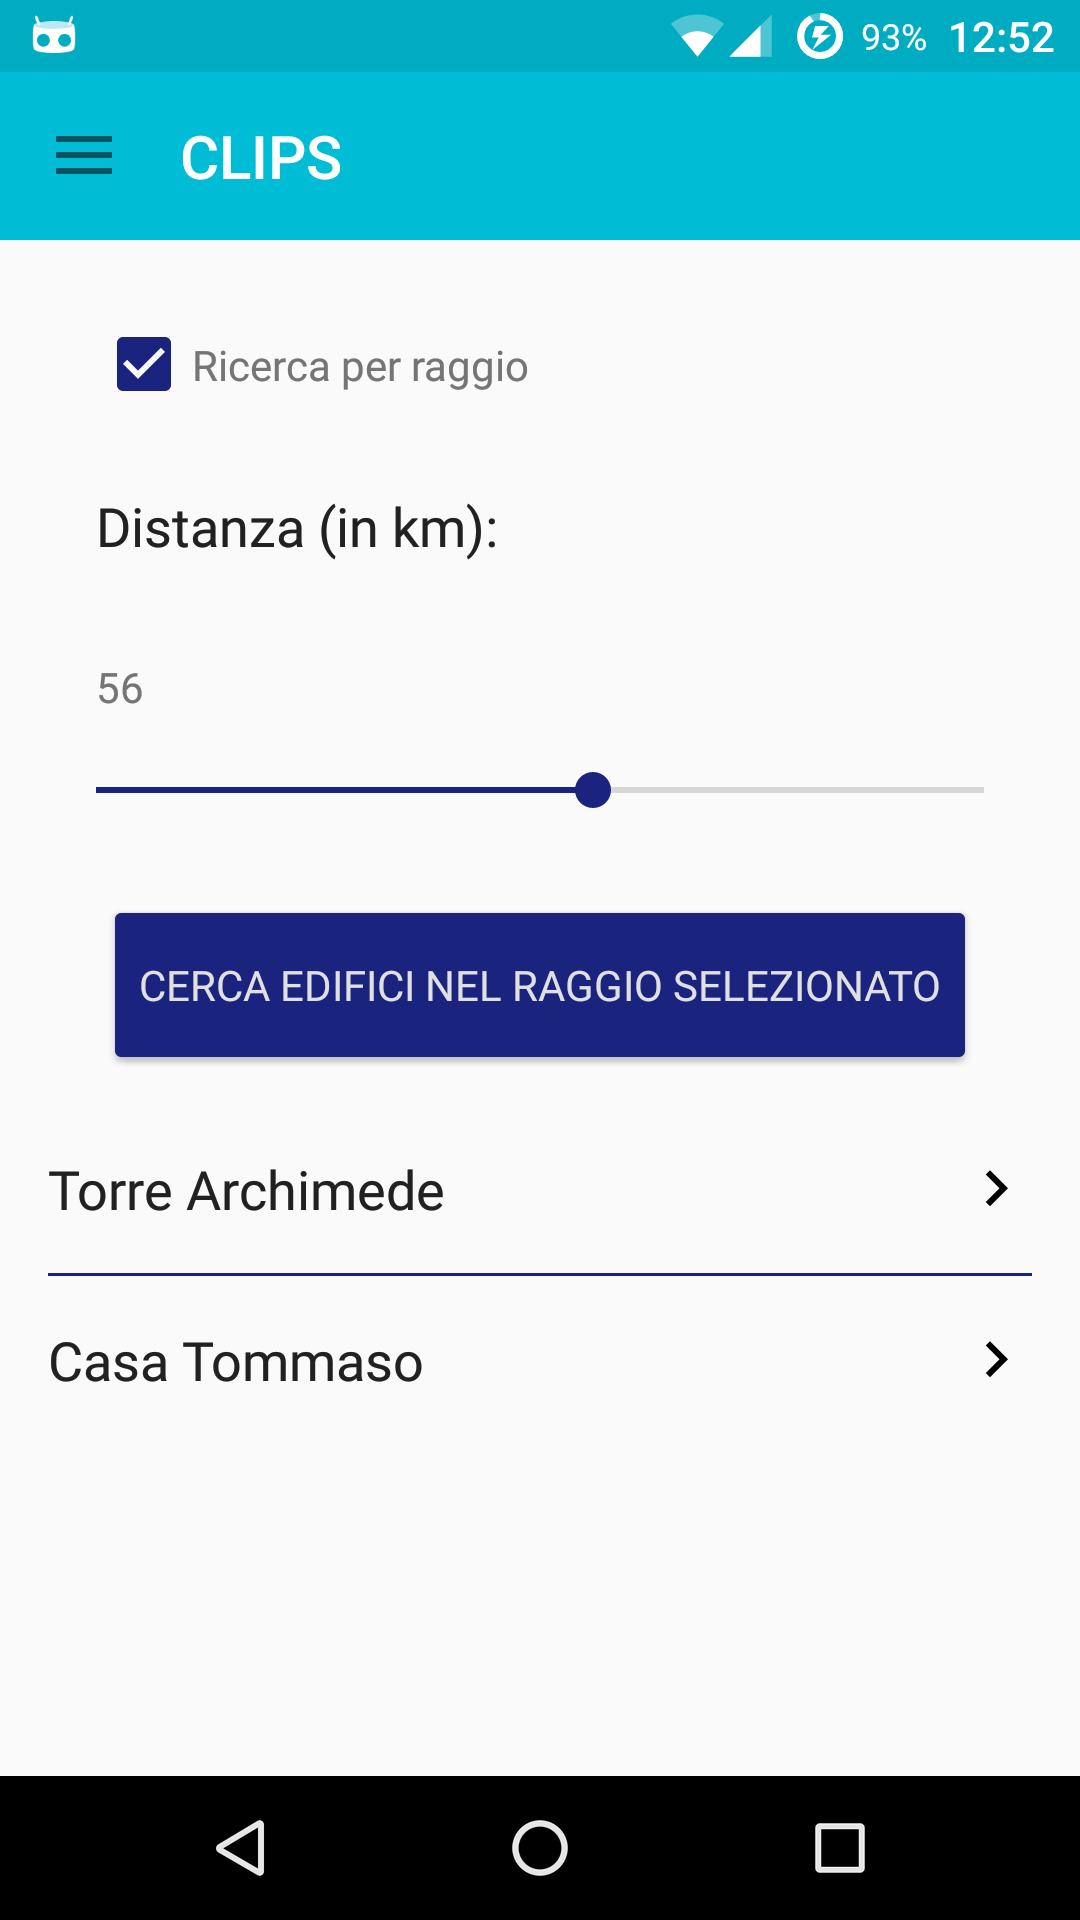
\includegraphics[scale=0.15]{screenshot/searchedifici}
	\caption{Schermata di ricerca edifici}
\end{figure}

\begin{figure}[!h]
	\centering
	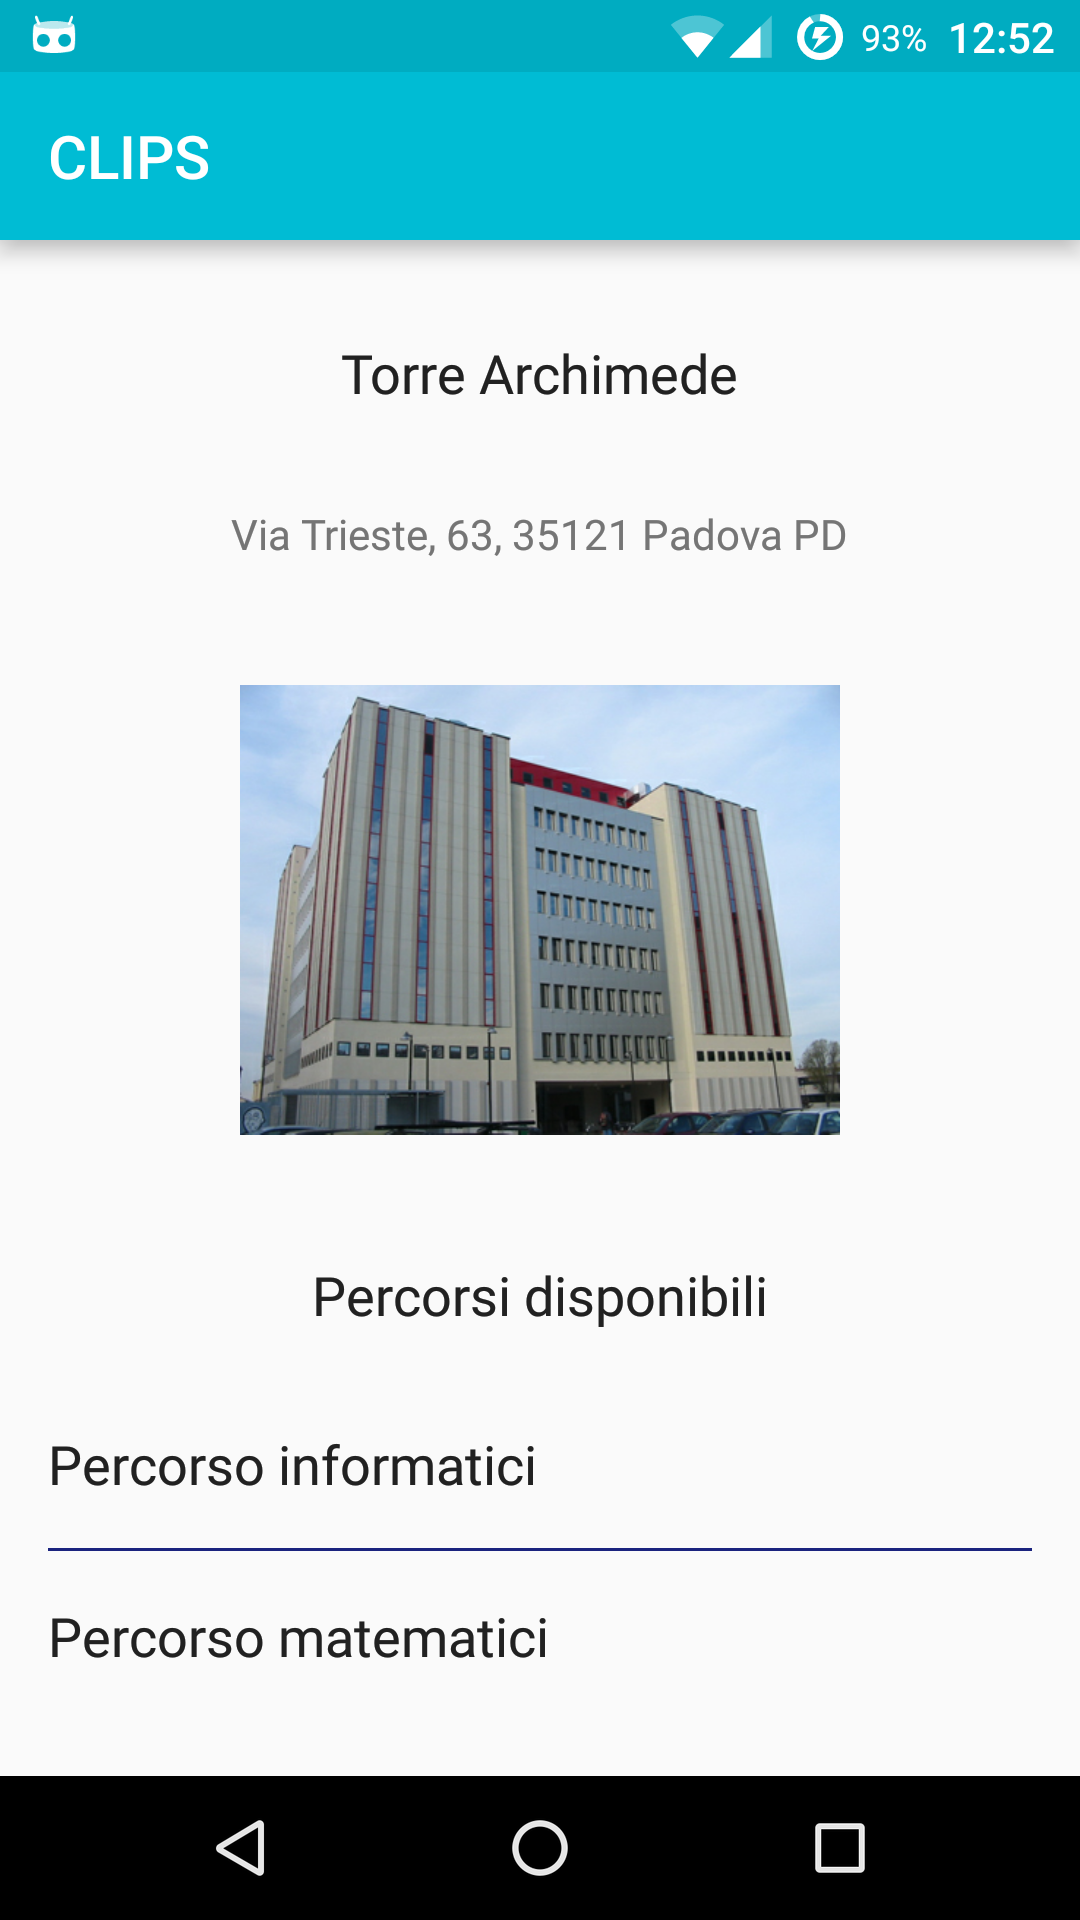
\includegraphics[scale=0.15]{screenshot/edificio}
	\caption{Schermata di dettaglio edificio}
\end{figure}

\section{Gioco}


\appendix
\newcommand{\lettera}[1]{
	\begin{center}
		{\Huge #1}\\
	\end{center}
	\rule{15cm}{0.4pt}
	\vspace{1cm}
}

\newcommand{\parola}[2]{
	\textbf{\large{#1}} \\
	\indent #2 
	\vspace{0.3cm}
}
\end{document}